\section{Compatibilità con i browser}
Per confermare la compatibilità e il medesimo grado di accessibilità, sono state testati più browser in modo da accertarsi della bontà di Auxils.it. Il sito mantiene lo stesso grado di accessibilità con tutti i browser testati, tutti gli script Javascript funzionano appieno su tutti i browser testati e le differenze sono presenti in minima parte in Internet Explorer solamente nella presentezione.\\
\subsection{Internet Explorer 6}
Vista la penuria di browser simulati dalla versione di prova di BrowserStack, ho dovuto affidarmi per la simulazione di Internet Explorer 6 ad IETester, un programma open source che permette di simulare Internet Explorer dalla versione 5.5 alla versione 11. Il problema di questa applicazione è che simula con un ottimo livello di stabilità solamente Internet Explorer 6, avendo ancora problemi con le altre versioni.\\
\begin{figure}[H]
  \centering 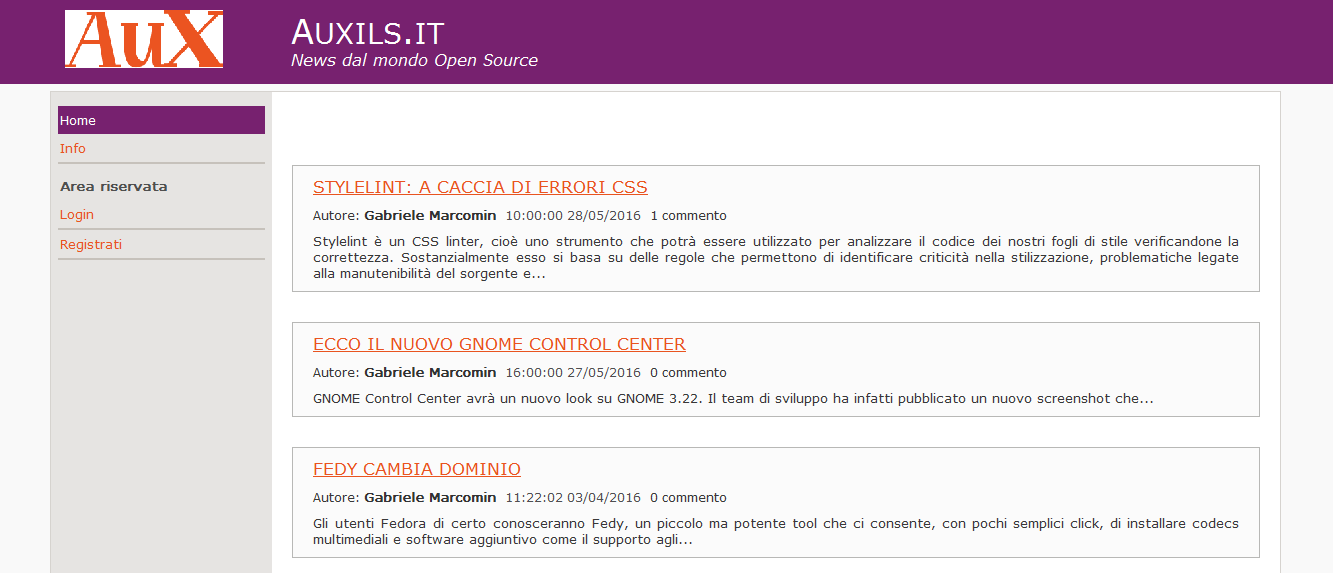
\includegraphics[width=0.6\textwidth]{images/homeie6.png}
  \caption{Home visualizzata simulando Internet Explorer 6}
\end{figure}
L'utilizzo di un esiguo numero di costrutti di CSS 3 ha permesso di avere da subito un sito portabile, accattivante ed accessibile allo stesso tempo, anche da browser non al passo coi tempi. Sono state usate comunque soluzioni utili ad aumentare la compatibilità con più browser possibili, mantenendo il medesimo aspetto grafico e grado di accessibilità.\\
Non sono state supportate le seguenti caratteristiche:
\begin{itemize}
  \item i bordi arrotondati non vengono visualizzati;
  \item il foglio di stile per risoluzioni inferiori a 480px non viene attivato;
  \item il bordo inferiore dell'ultimo elemento contenuti nella barra di navigazione viene comunque visualizzato;
  \item i pixel trasparenti del logo vengono sostituiti con pixel di colore bianco.
\end{itemize}
\begin{figure}[H]
  \centering 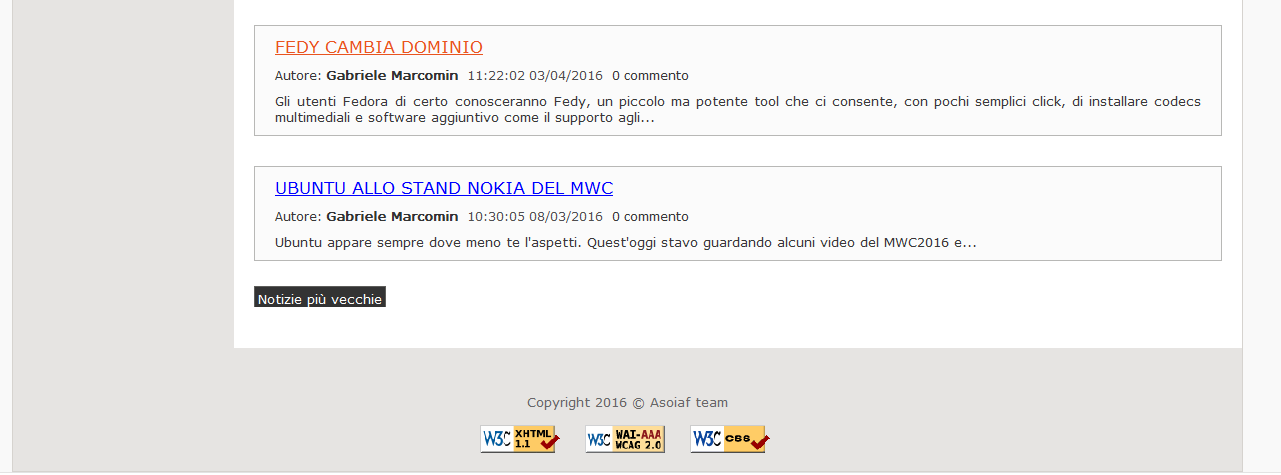
\includegraphics[width=0.6\textwidth]{images/homeie62.png}
  \caption{Footer visualizzato simulando Internet Explorer 6}
\end{figure}
\subsection{Altri browser}
Il sito è stato testato sulle ultime versioni di Microsoft Edge, Chrome, Firefox, Safari e su Internet Explorer 11 grazie a BrowserStack; il test ha potuto dimostrare la piena compatibilità di Auxils.it con i browser precedentemente elencati.